\documentclass[spanish,12pt]{elsarticle}
\usepackage{graphicx}
\usepackage{amssymb}
\usepackage{amsmath}
\usepackage{siunitx}
\usepackage{lineno}
\usepackage{babel}
\newcommand{\blank}[1]{\hspace*{#1}}
\makeatletter
\def\ps@pprintTitle{%
  \let\@oddhead\@empty
  \let\@evenhead\@empty
  \let\@oddfoot\@empty
  \let\@evenfoot\@oddfoot
}
\makeatother

\abstracttitle{Resumen}

\begin{document}

\begin{frontmatter}
\title{Problema K-minimum spanning tree}
\author{Roberto Juan Cayro Cuadros, Gabriel Alexander Valdivia Medina,
Giulia Alexa Naval Fernández, Rodrigo Alonso Torres Sotomayor}
\begin{abstract}
    El presente trabajo presenta una breve investigación del problema \textit{k-minimun spanning tree}, explicando su funcionamiento, demostrando que pertenece al conjunto de los problemas NP-completos, y dando opciones de algoritmos para su resolución.\\
\end{abstract}
\address{Universidad Católica San Pablo}

\end{frontmatter}

%%
%% Start line numbering here if you want
%%

%% main text
\section{Introducción al problema}
Según múltiples fuentes\cite{2}\cite{4}, el k-MST o k-minnimum spanning tree problem, árbol de expansión de péso mínimo k en español es un problema computacional que pide un árbol de mínimo costo con exactamente $k$ vértices que forme un subgrafo del grafo original.
\begin{figure}[h]
    \centering
    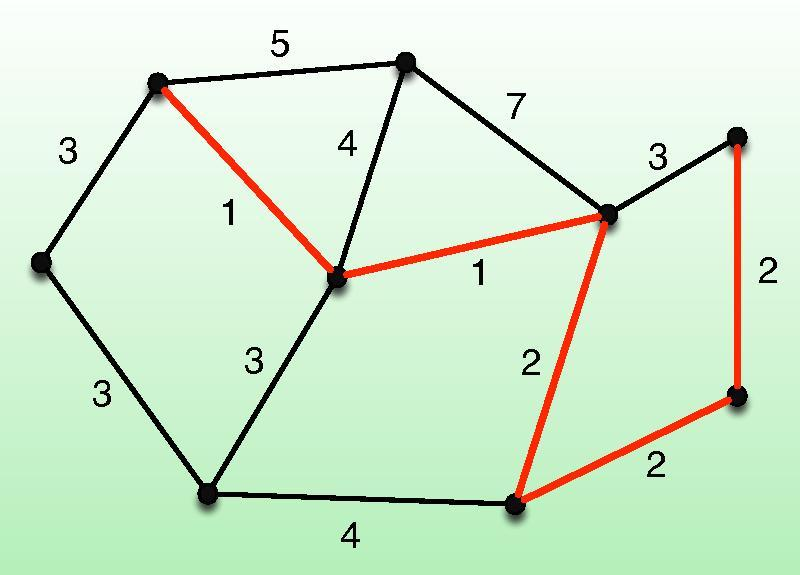
\includegraphics[scale=0.5]{images/6-mst.jpg}
    \caption{6-MST del grafo G. Fuente: Wikipedia Commons}
    \label{fig:my_label}
\end{figure}
%---------------------------------------------------------%


\section{Demostración NP-completo}
\paragraph{\textnormal{No es posible suponer la naturaleza del problema, y establecer que es NP-hard o NP-completo, sin la evidencia correspondiente, para probrarlo este debe pertenecer a NP, ademas que un problema NP-completo pueda reducirse al mismo}}
\subsection{Demostrar que k-MST $\in$ NP}
Para demostrar que un problema pertenece a la clase NP, se debe crear un algoritmo no deterministico que resuelva el problema en tiempo polinomial:\\\\
\textit{\underline{k-MST (G,k)} }

<<<<<<< HEAD
\begin{enumerate}
    \item \textnormal{x $\leftarrow$ arbol.}
=======
    \item \textnormal{x $\leftarrow$ árbol.}
    
>>>>>>> 0f2830b3751f31df7e39f42fa89949fd01a75e92
    \item  \textnormal{\textbf{for} t $\leftarrow$ 0,
    \textbf{to} k}
    \item \textnormal{\blank{1cm}\textbf{do} u $\leftarrow${ESCOGER(G)}}
    \item  \textnormal{\blank{2cm}\textbf{if} u \textbf{is not in} x}
    \item \textnormal{\blank{3cm}\textbf{do} x . add(u)}
\end{enumerate}



\subsection{Transformación NP-completo $\alpha$  k-MST}
El segundo paso para demostrar que un problema pertenece a los NP-completos, es transformar un problema NP-completo conocido para que pueda ser resuelto por el algoritmo del k-MST. Una transformación sencilla es la que se puede hacer dese el problema de Steiner.
\subsubsection{Steiner problem}
Según el artículo de Shivam Gupta\cite{1}, el Steiner problem es un problema NP-completo de los 21 problemas de Karp, usado en problemas de optimización y mayormente enfocado en estructuras de grafos aunque tambien visto en aplicaciones de modelación de redes con más de 2 terminales. El problema consiste en que, dado un grafo no-dirigido de aristas con peso, generar un arbol dado un
\textit{Sub-set} de vertices los cuales formarán este arbol. Además, pueden añadirse nuevos vertices del grafo al \textit{sub-set} para lograr las conexiones entre estos, llamados \textit{Steiner-vertices}.
\clearpage
La decisión asociada al problema será averiguar si existe un árbol que una todos los vértices de un \textit{sub-set} $R$, usando máximo $M$ aristas. Los vertices deberán ser exactamente los dados en el Sub-set. Esta decisión es conocida por ser del grupo de los NP-completos.
La principal diferencia con el k-MST es que aquí recibimos un conjunto específico de vectores para conformar nuestro árbol, pudiendo usar vértices fuera de la relación para conectarlos. El k-MST no recibe esta relación, sólo el número de vértices exactos que necesita.\\ 


\subsection{Entradas y salidas}


\subsubsection*{\underline{Steiner-problem}}
\begin{tabular}{ |l| }
\hline
Steiner-problem \\ \hline
\textit{Entrada: }\\
\blank{1cm} *Grafo no-dirigido G con aristas de peso. \\
\blank{1cm} *Sub-set de vertices R. \\
\blank{1cm} *Número M. \\

\\\hline
\textit{Salida: } \\
\blank{1cm} *Arbol de menor peso con los vertices de S \\
\blank{1cm}y los Steiner-vertices si fueran necesarios.\\
\\\hline
\end{tabular}

\subsubsection*{\underline{k-MST}}
\begin{tabular}{ |l| }
\hline
k-MST \\ \hline
\textit{Entrada: }\\
\blank{1cm} *Grafo no-dirigido G con aristas de peso. \\
\blank{1cm} *Número k de vértices. \\

\\\hline
\textit{Salida: } \\
\blank{1cm} *Arbol de menor peso con k-vertices y k-1, \\
\blank{1cm}aristas.\\

\\\hline
\end{tabular}

\subsubsection{Transformación}
\textnormal{Una primera aproximación será que dada la entrada G para Steiner, se puede tomar el mismo grafo para k-MST, puesto que tiene las aristas pesadas y un número determinado de vertices. De esta forma aseguramos la transformación y no afectara la salida porque siempre busaremos el arbol de menor peso , se usará el tamaño del sub-set de vertices siendo este igual a k.}\\\\
\textnormal{Pero no podemos asegurar que esta transformación pudiera también resolver al Steiner tree, siendo esta una de las propiedades en una transformación polinómica. Como tenemos de entrada un G, y k, podriamos calcular todas las permutaciones de G en k. Y necesariamente una de ellas corresponderia a la solución para Steiner:}\\\\
\textit{
\[
\textnormal{Total~de~permutaciones (Tn)}= \binom{n}{k} = \frac{n!}{k!(n - k)! }.
\]
}

\[
S \subseteq Tn.
\]
Sin embargo, calcular todas las permutaciones de una cantidad $n$ de elementos es un proceso con una complejidad $O(!n)$, que no entra dentro de complejidad polinomial, además que esta reducción planteada no resolverá el problema de k-MST, ya que este necesitaría solo 1 árbol de menor peso. Es necesario entonces otro tratamiento para que el k-MST opere con los vértices que el algoritmo Steiner pide. Siguiendo la transformación de R. Ravi \cite{3}, otra idea es añadir un árbol con aristas de peso 0 en cada vértice que pertenezca a R, y transformar $k$ como $k = |R|(X+1)$, siendo X la cantidad de vértices que tendrán cada uno de estos árboles, denotado como $X = |V(G)|-|R|$ De esta forma, el k-MST utilizará los vértices de $R$ sí o sí como parte de su solución.
\\\\ 
\begin{figure}[h]
    \centering
    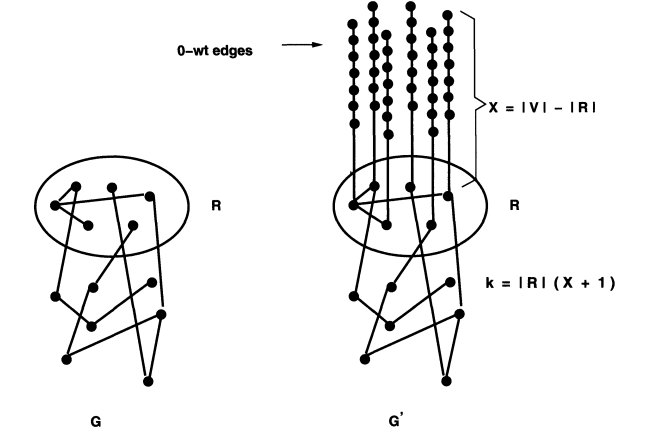
\includegraphics[scale=0.65]{images/graph_explicacion.png}
    \caption{Transformación de la entrada de Steiner a entrda de k-MST. Fuente: www.contrib.andrew.cmu.edu }
    \label{fig:my_label}
\end{figure}
\\
En este nuevo grafo $G'$, las aristas que unen los nuevos vértices de X tendrán un peso de 0, las aristas correspondientes a las aristas originales de G tendrán un peso de 1, y el resto de pares del grafo tendrán un peso de $\infty$. De este modo, el algoritmo del k-MST encontrará el árbol de menor peso con el parámetro k en $G'$, y verificará si es de igual o menor peso que M, satisfaciendo el requisito de las M aristas debido a que estas tendrán peso 1.\\


 
\section{Algoritmo de fuerza bruta}



\section{Algoritmo aproximado}



%% References
%%
%% Following citation commands can be used in the body text:
%% Usage of \cite is as follows:
%%   \cite{key}          ==>>  [#]
%%   \cite[chap. 2]{key} ==>>  [#, chap. 2]
%%   \citet{key}         ==>>  Author [#]

%% References with bibTeX database:

\bibliographystyle{model1-num-names}
\appendix
\section*{Bibliography}
\bibliography{sample.bib}

%% Authors are advised to submit their bibtex database files. They are
%% requested to list a bibtex style file in the manuscript if they do
%% not want to use model1-num-names.bst.

%% References without bibTeX database:

\begin{thebibliography}{00}
\bibitem{1} Gupta, S. (Junio de 2022). geeksforgeeks. Obtenido de https://www.geeksforgeeks.org/steiner-tree/
\bibitem{2}Matt Elder, S. C. (2007). CS880: Approximation Algorithms. Obtenido de https://pages.cs.wisc.edu/~shuchi/courses/880-S07/scribe-notes/lecture26-2.pdf
\bibitem{3}R. Ravi, R. S. (12 de Julio de 2006). Spanning Trees—Short or Small. Obtenido de SIAM (Society for Industrial and Applied Mathematics: https://epubs.siam.org/doi/pdf/10.1137/S0895480194266331
\bibitem{4} Wikipedia. (Junio de 2022). Wikipedia. Obtenido de https://en.wikipedia.org/wiki/K-minimum$_$spanning$_$tree


%% \bibitem must have the following form:
%%   \bibitem{key}...
%%

% \bibitem{}

\end{thebibliography}
%https://en.wikipedia.org/wiki/K-minimum_spanning_tree
%https://www.geeksforgeeks.org/steiner-tree/
%https://pages.cs.wisc.edu/~shuchi/courses/880-S07/scribe-notes/lecture26-2.pdf
%https://www.contrib.andrew.cmu.edu/~ravi/sidma96.pdf

\end{document}

%%
%% End of file `elsarticle-template-1-num.tex'.
